\tikzset{%
  block/.style    = {draw, rectangle, rounded corners=2pt, thin, minimum height = 2em, minimum width = 4em, fill=blue!10!white},
  sum/.style      = {draw, circle, node distance = 2cm}, % Adder
  io/.style    = {coordinate}, %input-output
    junction/.style    = {coordinate}
}
% Defining string as labels of certain blocks.
\newcommand{\suma}{\Large$+$}
\newcommand{\inte}{$\displaystyle \int$}
\newcommand{\derv}{\huge$\frac{d}{dt}$}

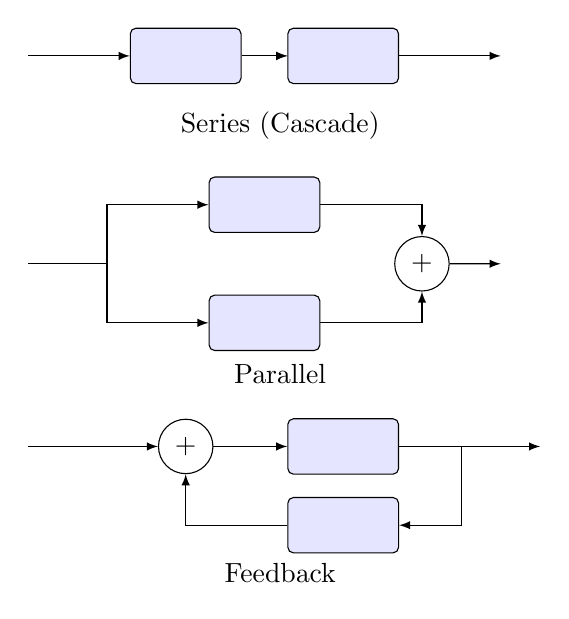
\begin{tikzpicture}[auto, node distance =2cm, scale=0.8]

	\begin{scope}
		\node (input) at (0,0) [io] {};
		\node (b1) [right of=input, block] {};
		\node (b2) [right of=b1, block] {};
		\node (output) [right of=b2, io] {};
		
		\draw[-latex](input) --  (b1);
		\draw[-latex](b1) --  (b2);
		\draw[-latex](b1) --  (b2); 	
		\draw[-latex](b2) --  (output);
		
		\node at (4, -1.1) {Series (Cascade)};		
	\end{scope}	
	
	\begin{scope}[yshift=-3.3cm]
		\node (input) at (0,0) [io] {};
		\node (j1) [right of=input, xshift=-1cm, junction] {};	
		\node (b1) [above of=j1, xshift=2cm, yshift=-1.25cm, block] {};
		\node (b2) [below of=j1, xshift=2cm, yshift=1.25cm, block] {};		
		\node (s1) [right of=b1, xshift=0cm, yshift=-0.75cm, sum] {$+$};				
		\node (output) [right of=s1, xshift=-1cm, io] {};
		
		
		\draw[] (input) --  (j1);		
		\draw[-latex] (j1) |-  (b1);	
		\draw[-latex] (j1) |-  (b2);	
		\draw[-latex] (b1) -|  (s1);	
		\draw[-latex] (b2) -|  (s1);
		\draw[-latex] (s1) --  (output);		
		\node at (4, -1.75) {Parallel};			
	\end{scope}
	
	
	\begin{scope}[yshift=-6.2cm]
		\node (input) at (0,0) [io] {};
		\node (s2) [right of=input, sum] {$+$};	
		\node (b3) [right of=s2, xshift=0cm, block] {};
		\node (j2) [right of=b3, xshift=-0.5cm,  junction] {};		
		\node (output) [right of=j2, xshift=-1cm, io] {};	
		\node (b4) [below of=b3, yshift=1cm, block] {};		

		
		
		\draw[-latex] (input) --  (s2);		
		\draw[-latex] (s2) --  (b3);	
		\draw[] (b3) --  (j2);
		
		\draw[-latex] (j2) --  (output);	
		\draw[-latex] (j2) |- (b4);		
		\draw[-latex] (b4) -| (s2);
		\node at (4, -2) {Feedback};			
	\end{scope}	
\end{tikzpicture} 